\documentclass[conference]{IEEEtran}
\usepackage[utf8]{inputenc}
\usepackage[T1]{fontenc}
\usepackage[spanish,es-tabla,es-noshorthands]{babel}
\usepackage{amsmath,amssymb}
\usepackage{graphicx}
\usepackage{booktabs}
\usepackage{multirow}
\usepackage{cite}
\usepackage{xcolor}
\usepackage[hidelinks]{hyperref}
\newcommand{\pend}[1]{\textcolor{red}{[#1]}}
\newcommand{\pmsd}[2]{$#1 \pm #2$}
\renewcommand{\IEEEkeywordsname}{Palabras clave}

\begin{document}

\title{¿Qué se puede recuperar del torque en la base de los bigotes? Localización de objetos y límites de la discriminación de forma en una matriz simulada de vibrisas de rata}

\author{\IEEEauthorblockN{Carolina Londoño Idárraga}
\IEEEauthorblockA{Máster en Inteligencia Artificial\\
Universitat Internacional Valenciana (VIU)\\
caroidarraga@gmail.com}
\and
\IEEEauthorblockN{Dr.-Ing. José Luis Zárate Moya}
\IEEEauthorblockA{Universitat Internacional Valenciana (VIU)\\
zarate.jl@gmail.com}}

\maketitle

\begin{abstract}
Los roedores localizan e identifican objetos con sus bigotes usando únicamente las señales mecánicas que llegan a la base de cada bigote. Estudiamos cuánta de la geometría de un objeto pueden recuperar modelos de aprendizaje a partir de esas señales. Con el simulador WHISKiT Physics generamos 1212 simulaciones nuevas de una matriz de 27 bigotes que bate activamente contra objetos, y registramos los tres momentos y las tres fuerzas en la base de cada bigote. Los modelos se evalúan con validación cruzada por simulación, normalización ajustada solo con entrenamiento, varias semillas aleatorias y modelos de referencia sin dinámica temporal. Para un poste vertical, una CNN--LSTM compacta recupera su posición en el plano con un error de \pmsd{1.76}{0.14}~mm, en empate estadístico con un bosque aleatorio sobre un mapa de contacto estático (\pmsd{1.71}{0.28}~mm), pero es mucho más robusta al ruido del sensor: con ruido del 20\,\% de la desviación estándar del canal su error se mantiene en 1,84~mm, mientras que el del bosque aleatorio sube a 5,65~mm. Para objetos de tres familias de forma, la posición se sigue recuperando (1,78--2,56~mm), pero la forma no: una vez que la forma del objeto se desacopla de su pose, todos los modelos quedan al nivel del azar, tanto con la cabeza quieta (exactitud de 0,39; azar 0,33) como con la cabeza avanzando hacia el objeto (0,38). Un clasificador de control que solo ve la pose del objeto deja al descubierto un atajo de diseño que, de otro modo, habría producido una exactitud aparente de 0,70. Concluimos que, en este régimen de contactos breves, el torque en la base de los bigotes contiene información robusta sobre dónde está un objeto, pero no sobre qué es, y que los controles de solo pose son necesarios en los bancos de prueba táctiles simulados.
\end{abstract}

\begin{IEEEkeywords}
percepción táctil, bigotes, vibrisas, señales de torque, WHISKiT Physics, CNN--LSTM, red convolucional temporal, aprendizaje por atajos
\end{IEEEkeywords}

\section{Introducción}
Las ratas exploran su entorno moviendo los bigotes de la cara hacia adelante y hacia atrás varias veces por segundo, un comportamiento conocido como batido (\emph{whisking})~\cite{mitchinson2011}. Un bigote no tiene sensores a lo largo de su longitud: todo lo que el animal aprende de un objeto le llega como fuerzas y momentos en la base del bigote, dentro del folículo. Esto hace del sistema de vibrisas un modelo atractivo para el tacto robótico en condiciones en las que la visión falla, y ha motivado una línea de sensores artificiales tipo bigote que miden el torque en la base~\cite{kaneko1998,solomon2006,pearson2011,lepora2018}.

Para un solo bigote en régimen cuasiestático, la mecánica se conoce bien: el cociente entre el momento y la fuerza en la base determina la distancia radial de un contacto~\cite{kaneko1998,birdwell2007}, y la combinación de varias señales mecánicas da la posición tridimensional del contacto~\cite{huet2017}. Solomon y Hartmann usaron este principio para extraer rasgos de objetos con bigotes robóticos~\cite{solomon2006}. Se sabe mucho menos sobre qué puede decodificarse de una matriz completa durante el batido activo, donde los contactos son breves, los bigotes tienen inercia y decenas de ellos interactúan con el objeto al mismo tiempo. El simulador WHISKiT Physics~\cite{zweifel2021} modela esta situación para la matriz de la rata y devuelve la señal mecánica completa en la base de cada bigote, lo que permite plantear la decodificación como un problema de aprendizaje supervisado.

Este artículo plantea una pregunta deliberadamente simple: dados los momentos y las fuerzas en la base de 27 bigotes durante el batido activo, ¿qué propiedades de un objeto puede recuperar un modelo de aprendizaje y cuáles no? Presentamos un conjunto nuevo de experimentos diseñado para este estudio. Las contribuciones son:
\begin{itemize}
\item Un flujo de trabajo reproducible que convierte WHISKiT Physics en un generador de conjuntos de datos de torque etiquetados, con control desde la línea de comandos de la posición, la orientación y la escala del objeto y del movimiento de la cabeza.
\item Un resultado de localización: la posición en el plano de un poste se recupera con un error inferior a 2~mm, y se muestra que un modelo temporal es mucho más robusto al ruido del sensor que un resumen estático del contacto, aunque ambos son igual de precisos con datos limpios.
\item Un resultado negativo con dos réplicas independientes: la forma de objetos pequeños no puede discriminarse a partir de estas señales, ni con la cabeza quieta ni con la cabeza acercándose al objeto.
\item Un hallazgo metodológico: un clasificador de control que solo ve la pose revela que una forma natural de generar poses válidas acopla la forma a la posición e infla la exactitud de forma desde el azar hasta 0,70.
\end{itemize}

\section{Trabajo relacionado}
\subsection{Señales mecánicas en la base del bigote}
Kaneko \emph{et al.} mostraron que una viga flexible movida activamente, con un sensor de torque en su base, puede localizar un contacto a lo largo de su longitud~\cite{kaneko1998}. Birdwell \emph{et al.} derivaron modelos biomecánicos que relacionan la tasa de cambio del momento con la distancia radial de contacto en bigotes cónicos de rata~\cite{birdwell2007}, y Huet \emph{et al.} mostraron qué combinaciones de señales en la base determinan el punto de contacto tridimensional para bigotes de distintas formas~\cite{huet2017}. Estos trabajos analizan un solo bigote bajo flexión cuasiestática. Las implementaciones robóticas van desde matrices de bigotes con sensores de torque~\cite{solomon2006,pearson2011} hasta bigotes táctiles ópticos~\cite{lepora2018}.

\subsection{Simulación de la matriz de bigotes}
WHISKiT Physics~\cite{zweifel2021} representa cada bigote como una cadena de eslabones rígidos unidos por resortes de torsión dentro del motor de física Bullet~\cite{coumans2015}, con la morfología de la matriz de la rata promedio. Dada la cinemática del batido en la base (ángulos de protracción, elevación y giro), devuelve las tres componentes del momento y de la fuerza en la base de cada bigote. Lo usamos como fuente de datos y no modificamos su modelo mecánico.

\subsection{Aprendizaje a partir de series temporales táctiles}
Las redes recurrentes con memoria de corto y largo plazo (LSTM)~\cite{hochreiter1997} y los modelos convolucionales de secuencias, como las redes convolucionales temporales (TCN)~\cite{bai2018}, son opciones habituales para series temporales multicanal. Hay dos riesgos propios de la evaluación con datos simulados. El primero es la fuga de información entre entrenamiento y prueba, por ejemplo mediante estadísticas de normalización calculadas con todos los datos o mediante ventanas solapadas de un mismo registro~\cite{kapoor2023}. El segundo es el aprendizaje por atajos: un modelo puede alcanzar una exactitud alta explotando una regularidad del conjunto de datos que no tiene relación con la propiedad de interés~\cite{geirhos2020}. Nuestro protocolo está diseñado contra el primero, y la Sección~\ref{sec:shape} documenta un caso del segundo.

\section{Métodos}
\subsection{Configuración de la simulación}
Todos los datos se generaron con WHISKiT Physics usando el modelo de rata promedio, los 27 bigotes del lado derecho de la cara (filas A--E) y la trayectoria de batido activo que se distribuye con el simulador, cuya frecuencia es de 8~Hz. Las señales se registran a 1~kHz. Las coordenadas se expresan en el marco de la cabeza, en milímetros, con $x$ apuntando en dirección rostral e $y$ en dirección lateral hacia la derecha; las bases de los bigotes están cerca de $x\approx 6$~mm y las puntas de la matriz en reposo llegan a $x\approx 48$~mm.

Añadimos al simulador opciones de línea de comandos para fijar la posición del poste; la posición, el giro (\emph{yaw}) y la escala de un objeto arbitrario dado como malla; y una trayectoria de la cabeza dada como velocidades lineales y angulares por paso de tiempo. Los cinco primeros pasos de cada simulación contienen un transitorio numérico y se descartan. Los momentos y las fuerzas se reportan en las unidades nativas del simulador.

Cada simulación produce una muestra: un tensor de tamaño $T\times 27\times 6$ con canales $(M_x,M_y,M_z,F_x,F_y,F_z)$, donde $x$ es el eje del bigote en la base, de modo que $M_x$ es la torsión y $M_y$, $M_z$ son los momentos de flexión. La Fig.~\ref{fig:signals} muestra un ejemplo. Se considera que una simulación contiene contacto cuando el mayor momento absoluto sobre todos los bigotes y pasos de tiempo es de al menos 0,6; las simulaciones por debajo de ese umbral se reportan y se excluyen de la evaluación de los modelos.

\begin{figure}[t]
\centering
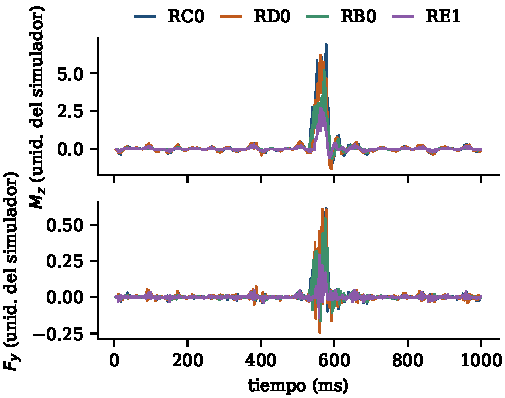
\includegraphics[width=\columnwidth]{figs_es/fig_signals.pdf}
\caption{Ejemplo de las señales de una simulación del conjunto~P (poste en $x=14{,}0$, $y=12{,}7$~mm): momento de flexión $M_z$ y fuerza transversal $F_y$ en la base de los cuatro bigotes con contacto más fuerte durante 1~s de batido (ocho ciclos).}
\label{fig:signals}
\end{figure}

\subsection{Conjuntos de datos}
La Tabla~\ref{tab:datasets} resume los cuatro conjuntos de datos.

\textbf{Conjunto P (localización del poste).} Un poste vertical fijo se coloca en una posición muestreada de forma uniforme en $x\in[12,42]$~mm, $y\in[9,31]$~mm, excluyendo dos esquinas que la matriz no alcanza. La etiqueta es la posición $(x,y)$ del poste.

\textbf{Conjuntos D1--D3 (forma y posición).} El objeto es una de nueve mallas de tres familias (cilindro, prisma rectangular, pared con frente sinusoidal), con tres tamaños cada una, colocada con posición y giro aleatorios. Las etiquetas son la familia de forma y la posición. Antes de simular, cada pose candidata se comprueba geométricamente con la huella de los bigotes en reposo y a lo largo de un ciclo de batido: una pose se rechaza si el objeto atraviesa un bigote en reposo, lo que iniciaría la simulación en penetración, o si el barrido del batido nunca alcanza el objeto.

Los tres conjuntos difieren en cómo se asignan las poses:
\begin{itemize}
\item \textbf{D1 (cabeza quieta, forma acoplada a la pose).} Se muestrean juntas una malla y una pose, y el par se acepta si es válido. Los tamaños difieren mucho entre familias (cilindros de 1 a 5~mm de radio, prismas de hasta $6\times20$~mm, paredes de hasta 25~mm de largo).
\item \textbf{D2 (cabeza quieta, forma desacoplada).} Primero se muestrea la pose y solo se acepta si es válida para las nueve mallas; después se asigna la malla al azar de forma balanceada. Las familias tienen tamaños comparables (cilindros de 4 a 6~mm de radio; prismas de $8\times8$, $6\times12$ y $10\times10$~mm; paredes de 12~mm de largo con amplitudes de 1,5 a 2,5~mm) y todos los objetos miden 160~mm de alto para que todas las filas de bigotes puedan alcanzarlos.
\item \textbf{D3 (cabeza avanzando, forma desacoplada).} Como D2, pero la cabeza avanza hacia el objeto a 60~mm/s, unos 28~mm durante la simulación, de modo que los bigotes se presionan contra el objeto en lugar de rozarlo con las puntas. Además, las poses deben mantener el objeto por delante de la cabeza en todo momento.
\end{itemize}

\begin{table}[t]
\caption{Conjuntos de datos generados para este estudio}
\label{tab:datasets}
\centering
\setlength{\tabcolsep}{3.5pt}
\begin{tabular}{@{}lcccc@{}}
\toprule
 & P & D1 & D2 & D3 \\
\midrule
Objeto & poste & 9 mallas & 9 mallas & 9 mallas \\
Cabeza & quieta & quieta & quieta & avanzando \\
Forma indep. de la pose & -- & no & sí & sí \\
Simulaciones & 300 & 300 & 306 & 306 \\
Duración (s) & 1,0 & 1,0 & 0,5 & 0,5 \\
Con contacto & 283 & 284 & 272 & 275 \\
Mediana del momento máx. & 4,5 & 2,2 & 1,5 & 2,7 \\
\bottomrule
\end{tabular}
\end{table}

\subsection{Modelos}
\textbf{CNN--LSTM.} Dos convoluciones unidimensionales sobre el tiempo (64 filtros, núcleo de 5, normalización por lotes, ReLU) seguidas de \emph{max pooling}, una LSTM bidireccional con 64 unidades por dirección, promedio temporal y una cabeza de dos capas. Tiene 148 mil parámetros. Los 162 canales de entrada son los 27 bigotes por seis señales.

\textbf{TCN.} Cinco niveles convolucionales con núcleo de 5 y dilataciones de 1, 2, 4, 8 y 16 (64 filtros, normalización por lotes, ReLU, \emph{dropout} de 0,2), seguidos de promedio temporal y la misma cabeza (139 mil parámetros). Como las simulaciones completas se analizan fuera de línea, las convoluciones no son causales.

\textbf{Modelos de referencia sin dinámica temporal.} (i) La media o la clase mayoritaria del entrenamiento. (ii) Regresión \emph{ridge} sobre la media, la desviación estándar y el máximo absoluto de cada canal. (iii) Un bosque aleatorio (\emph{random forest}, RF)~\cite{breiman2001} con 400 árboles sobre el \emph{mapa de contacto}, es decir, el máximo momento absoluto de cada bigote durante la simulación, que descarta toda la estructura temporal.

\textbf{Control de solo pose.} Para la clasificación de forma entrenamos además un bosque aleatorio que recibe únicamente la pose real del objeto $(x,y,\text{giro})$ y nunca ve las señales mecánicas. No es un competidor: su exactitud mide cuánto de la etiqueta de forma puede adivinarse por dónde está el objeto, es decir, el tamaño de cualquier atajo introducido por el diseño de los datos.

Para forma y posición las redes tienen dos cabezas, tres \emph{logits} para la familia de forma y dos salidas para la posición, entrenadas con entropía cruzada más diez veces el error cuadrático medio. El giro no se predice porque no está definido de forma única para cilindros y prismas simétricos.

\subsection{Protocolo de evaluación}
La unidad de partición es la simulación. Usamos validación cruzada de cinco pliegues (estratificada por clase en D1--D3); dentro de cada pliegue de entrenamiento se reserva el 20\,\% de las simulaciones para la parada temprana, y el pliegue de prueba se evalúa una sola vez. Cada canal se estandariza con la media y la desviación estándar de las simulaciones de entrenamiento únicamente. Las redes se entrenan con Adam~\cite{kingma2015} (tasa de aprendizaje $10^{-3}$, decaimiento de pesos $10^{-4}$, lotes de 8), reducción de la tasa de aprendizaje en meseta y parada temprana, y cada pliegue se repite con varias semillas aleatorias (tres en el conjunto~P, dos en los demás). Las etiquetas de posición se dividen entre 50~mm para el entrenamiento. Salvo indicación contraria, las señales se submuestrean a 500~Hz. Reportamos el error euclídeo medio de posición en milímetros y la exactitud de clasificación, como media~$\pm$~desviación estándar entre pliegues y semillas.

La robustez se mide evaluando modelos entrenados con datos limpios sobre simulaciones de prueba perturbadas: ruido gaussiano aditivo con desviación estándar igual al 5, 10 o 20\,\% de la desviación estándar de entrenamiento de cada canal, escalado de amplitud por 0,8 o 1,2 y desfases temporales de $\pm5$ muestras.

\section{Resultados}
\subsection{Localización del poste}
La Tabla~\ref{tab:peg} da el error de posición en las 283 simulaciones del conjunto~P con contacto. A 500~Hz, la CNN--LSTM alcanza \pmsd{1.76}{0.14}~mm y el bosque aleatorio sobre el mapa de contacto \pmsd{1.71}{0.28}~mm, frente a 9,47~mm de la media de entrenamiento y 3,77~mm de la regresión \emph{ridge}. Los dos mejores modelos son estadísticamente indistinguibles; la red tiene menor dispersión entre pliegues. Para la CNN--LSTM, el coeficiente de determinación es de 0,95 en $x$ y de 0,94 en $y$. La Fig.~\ref{fig:scatter} muestra las predicciones en el espacio de trabajo: la mediana del error es de 1,16~mm y los errores mayores aparecen en el borde de la región alcanzable. Las 17 simulaciones restantes no tuvieron contacto y ningún modelo puede localizarlas; marcan el límite de observabilidad de la matriz.

\begin{table}[t]
\caption{Localización del poste: error de posición (mm) según la frecuencia de muestreo}
\label{tab:peg}
\centering
\setlength{\tabcolsep}{4pt}
\begin{tabular}{@{}lccc@{}}
\toprule
Modelo & 100 Hz & 200 Hz & 500 Hz \\
\midrule
Media de entrenamiento & \pmsd{9.47}{0.45} & \pmsd{9.47}{0.45} & \pmsd{9.47}{0.45} \\
\emph{Ridge} sobre estadísticas & \pmsd{3.84}{0.58} & \pmsd{3.85}{0.39} & \pmsd{3.77}{0.72} \\
RF sobre mapa de contacto & \pmsd{1.97}{0.28} & \pmsd{1.87}{0.33} & \pmsd{1.71}{0.28} \\
CNN--LSTM & \pmsd{2.15}{0.18} & \pmsd{2.08}{0.22} & \pmsd{1.76}{0.14} \\
\bottomrule
\end{tabular}
\end{table}

\begin{figure}[t]
\centering
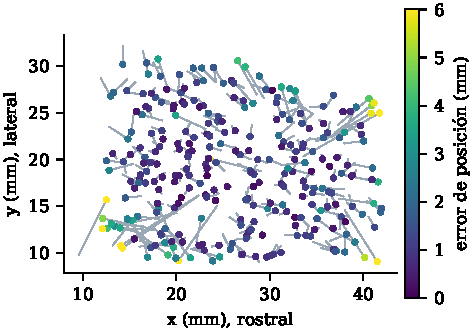
\includegraphics[width=\columnwidth]{figs_es/fig_scatter.pdf}
\caption{Localización del poste con la CNN--LSTM a 500~Hz (predicciones de prueba de todos los pliegues, una semilla). Cada punto es la posición real del poste, coloreada según el error; la línea lo une con la posición predicha.}
\label{fig:scatter}
\end{figure}

\textbf{Arquitectura y pérdida.} La Tabla~\ref{tab:ablation} compara variantes bajo un protocolo común. Todos los modelos compactos quedan entre 1,4 y 1,9~mm y sus diferencias son del orden de la variación entre pliegues. La TCN es la más precisa (\pmsd{1.44}{0.32}~mm), y el error cuadrático medio (MSE) es mejor pérdida que la L1 suavizada en esta escala de etiquetas. Una pérdida que añade al error cuadrático medio un término de similitud estructural (SSIM) unidimensional~\cite{wang2004} es inestable para una salida de dos dimensiones: dos de diez corridas divergieron. El tamaño del modelo no se tradujo en precisión: una variante con tres capas LSTM bidireccionales apiladas de 512, 256 y 128 unidades (6,4 millones de parámetros), evaluada en un solo pliegue a 200~Hz por su costo, alcanzó 3,48~mm, frente a unos 2,0~mm de la CNN--LSTM compacta en ese mismo pliegue, con aproximadamente 120 veces más tiempo de entrenamiento.

\begin{table}[t]
\caption{Localización del poste: variantes de arquitectura y de pérdida (500 Hz, cinco pliegues, dos semillas)}
\label{tab:ablation}
\centering
\begin{tabular}{@{}llcc@{}}
\toprule
Modelo & Pérdida & Error (mm) & Parámetros \\
\midrule
TCN & L1 suavizada & \pmsd{1.44}{0.32} & 139 mil \\
CNN--LSTM & MSE & \pmsd{1.54}{0.16} & 148 mil \\
Solo BiLSTM & L1 suavizada & \pmsd{1.76}{0.27} & 125 mil \\
CNN--LSTM & L1 suavizada & \pmsd{1.81}{0.19} & 148 mil \\
Solo CNN & L1 suavizada & \pmsd{1.84}{0.16} & 77 mil \\
CNN--LSTM & MSE + SSIM & mediana 1,95$^{\ast}$ & 148 mil \\
\bottomrule
\multicolumn{4}{@{}l}{\footnotesize $^{\ast}$Dos de diez corridas divergieron (errores de 10 y 38 mm).}
\end{tabular}
\end{table}

\textbf{Robustez.} La Tabla~\ref{tab:robust} y la Fig.~\ref{fig:noise} muestran la principal diferencia entre el modelo temporal y el resumen estático. El error de la CNN--LSTM no cambia con ruido aditivo de hasta el 20\,\% de la desviación estándar del canal (1,84~mm), mientras que el bosque aleatorio sobre el mapa de contacto se degrada hasta 5,65~mm, un factor de 3,3. El mapa de contacto se construye con máximos, que el ruido sesga hacia arriba, mientras que la red integra toda la secuencia. El escalado de amplitud afecta a ambos modelos de forma parecida, y ninguno es sensible a un desfase de $\pm5$ muestras; el mapa de contacto es invariante a los desfases por construcción.

\begin{table}[t]
\caption{Localización del poste: error de posición (mm) con perturbaciones en la prueba (500 Hz, cinco pliegues)}
\label{tab:robust}
\centering
\begin{tabular}{@{}lcc@{}}
\toprule
Condición & CNN--LSTM & RF sobre mapa de contacto \\
\midrule
Limpio & \pmsd{1.84}{0.20} & \pmsd{1.71}{0.28} \\
Ruido 5\,\% & \pmsd{1.84}{0.19} & \pmsd{2.41}{0.34} \\
Ruido 10\,\% & \pmsd{1.84}{0.19} & \pmsd{3.75}{0.47} \\
Ruido 20\,\% & \pmsd{1.84}{0.17} & \pmsd{5.65}{0.61} \\
Amplitud $\times0.8$ & \pmsd{2.34}{0.25} & \pmsd{2.21}{0.25} \\
Amplitud $\times1.2$ & \pmsd{2.04}{0.18} & \pmsd{2.62}{0.16} \\
Desfase de $+5$ muestras & \pmsd{1.86}{0.19} & \pmsd{1.71}{0.28} \\
Desfase de $-5$ muestras & \pmsd{1.90}{0.21} & \pmsd{1.71}{0.28} \\
\bottomrule
\end{tabular}
\end{table}

\begin{figure}[t]
\centering
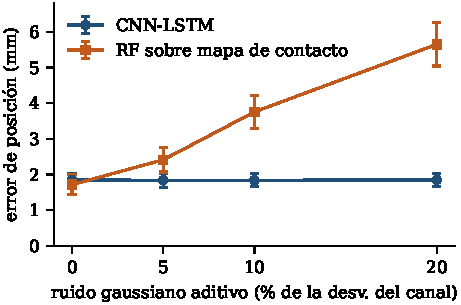
\includegraphics[width=\columnwidth]{figs_es/fig_noise.pdf}
\caption{Error de posición en el conjunto~P en función del ruido aditivo en la prueba. Las barras de error son la desviación estándar entre pliegues.}
\label{fig:noise}
\end{figure}

\subsection{Forma y posición de objetos}
\label{sec:shape}
La Tabla~\ref{tab:shape} y la Fig.~\ref{fig:shape} presentan los resultados en D1--D3.

\textbf{Un atajo de diseño (D1).} En D1 los modelos parecen reconocer la forma: el bosque aleatorio alcanza una exactitud de 0,70 y la CNN--LSTM de 0,68. El control de solo pose, que nunca ve las señales, alcanza 0,62. La comprobación geométrica de validez había atado la forma a la posición, porque los objetos más grandes solo caben más lejos de la cabeza: la $x$ media fue de 39,7~mm para los cilindros, 40,6~mm para los prismas y 43,5~mm para las paredes. Los modelos con torque aportan solo entre 3 y 8 puntos sobre ese control, y la mayor parte de lo que parece reconocimiento de forma es reconocimiento de dónde está el objeto.

\textbf{Diseño desacoplado, cabeza quieta (D2).} Cuando las poses son válidas para todas las mallas y la malla se asigna después, el control de solo pose cae al azar (\pmsd{0.36}{0.07}; 0,29 calculado sobre la lista de poses antes de simular). Entonces ningún modelo se separa del azar: 0,39 tanto para el bosque aleatorio como para la CNN--LSTM, y 0,37 para la TCN, con matrices de confusión repartidas por igual entre las tres clases.

\textbf{Diseño desacoplado, cabeza avanzando (D3).} Mover la cabeza hacia el objeto eleva la mediana del momento máximo de 1,5 a 2,7 y los valores más altos de unos 5 a 14, de modo que los contactos ya no se limitan a las puntas de los bigotes. La exactitud de forma no cambia: 0,36 para el bosque aleatorio y 0,38 para ambas redes, frente a 0,36 del control de solo pose. Un bosque aleatorio con descriptores más ricos por canal (media, desviación estándar, extremos, instante del pico y mayor incremento) alcanza \pmsd{0.39}{0.05}. Restringir el análisis a las 93 simulaciones con contacto más fuerte da \pmsd{0.44}{0.10}, y el problema binario de cilindro frente a pared en simulaciones de contacto fuerte da \pmsd{0.61}{0.12}, con un nivel de azar de 0,50. Estos valores sugieren una dependencia débil de la intensidad del contacto, pero están dentro de la variación entre pliegues.

\textbf{Posición.} En cambio, la posición del objeto se recupera en los tres conjuntos. El bosque aleatorio sobre el mapa de contacto da \pmsd{1.78}{0.11}~mm en D2 y \pmsd{2.56}{0.17}~mm en D3, donde el rango de posiciones es más amplio y el error de la media de entrenamiento es de 11,15~mm. Las redes son menos precisas que el bosque aleatorio en estos conjuntos (3,1--5,9~mm), que tienen unas 220 simulaciones de entrenamiento por pliegue y una señal más débil que la del conjunto~P.

\begin{table}[t]
\caption{Exactitud de forma (azar: 0,333) y error de posición para objetos de tres familias de forma}
\label{tab:shape}
\centering
\setlength{\tabcolsep}{3.5pt}
\begin{tabular}{@{}lccc@{}}
\toprule
 & D1 & D2 & D3 \\
\midrule
\multicolumn{4}{@{}l}{\emph{Exactitud de forma}} \\
Clase mayoritaria & 0,35 & 0,35 & 0,34 \\
Control de solo pose & \pmsd{0.62}{0.05} & \pmsd{0.36}{0.07} & \pmsd{0.36}{0.06} \\
RF sobre mapa de contacto & \pmsd{0.70}{0.03} & \pmsd{0.39}{0.08} & \pmsd{0.36}{0.04} \\
CNN--LSTM & \pmsd{0.68}{0.08} & \pmsd{0.39}{0.05} & \pmsd{0.38}{0.04} \\
TCN & \pmsd{0.65}{0.08} & \pmsd{0.37}{0.04} & \pmsd{0.38}{0.05} \\
\midrule
\multicolumn{4}{@{}l}{\emph{Error de posición (mm)}} \\
Media de entrenamiento & \pmsd{4.94}{0.29} & \pmsd{7.07}{0.79} & \pmsd{11.15}{0.79} \\
RF sobre mapa de contacto & \pmsd{3.30}{0.27} & \pmsd{1.78}{0.11} & \pmsd{2.56}{0.17} \\
CNN--LSTM & \pmsd{4.11}{0.30} & \pmsd{3.15}{0.60} & \pmsd{5.11}{0.57} \\
TCN & \pmsd{5.31}{1.08} & \pmsd{3.90}{0.70} & \pmsd{5.88}{0.73} \\
\bottomrule
\end{tabular}
\end{table}

\begin{figure}[t]
\centering
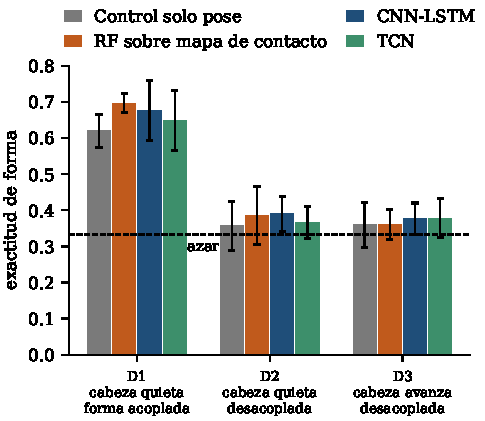
\includegraphics[width=\columnwidth]{figs_es/fig_shape.pdf}
\caption{Exactitud de forma en los tres diseños. En D1, el control de solo pose, que no ve las señales mecánicas, ya alcanza 0,62. Una vez que la forma es independiente de la pose (D2, D3), todos los modelos quedan en el azar, con la cabeza quieta o avanzando.}
\label{fig:shape}
\end{figure}

\section{Discusión}
\textbf{Dónde frente a qué.} Las señales en la base de la matriz contienen información robusta sobre la posición del objeto. Un resumen estático, el mayor momento visto por cada bigote, basta para ubicar un poste con menos de 2~mm de error, lo que concuerda con la visión clásica en la que el patrón de qué bigotes tocan y con cuánta fuerza codifica la localización~\cite{kaneko1998,birdwell2007}. La forma es un asunto distinto. Las tres familias usadas aquí difieren en unos pocos milímetros a la escala de un solo objeto, mientras que los bigotes vecinos están separados por varios milímetros y cada contacto dura una fracción de un ciclo de batido. Con la cabeza quieta, los objetos deben quedar más allá del alcance de la matriz en reposo para evitar la penetración inicial, así que solo los tocan las puntas de los bigotes; con la cabeza avanzando, el contacto es más fuerte, pero sigue siendo una secuencia corta de toques con una orientación desconocida. En ambos regímenes, las señales de las tres familias no son separables por ninguno de los modelos probados, incluido uno que solo resume el contacto y dos que usan la dinámica completa. Por eso atribuimos el resultado al contenido de información de la señal en este régimen de contacto y no a la capacidad de los modelos.

\textbf{Cuándo importan los modelos temporales.} Con datos limpios, modelar la dinámica no mejoró la localización respecto al mapa de contacto, y todas las arquitecturas compactas rindieron de forma parecida. El beneficio del modelo temporal aparece con ruido en el sensor, donde conserva su precisión y el resumen basado en máximos no. Para un sensor físico, esta es la comparación más relevante.

\textbf{Controles de solo pose.} El atajo de D1 surgió de un paso razonable, rechazar las poses inválidas para cada objeto, y habría pasado inadvertido en una evaluación estándar, porque la exactitud estaba muy por encima del azar y la matriz de confusión parecía plausible. Un clasificador que solo ve las variables de confusión se entrena en segundos, puede ejecutarse sobre la lista de poses antes de cualquier simulación y acota cuánto de un resultado puede ser un atajo~\cite{geirhos2020}. Sugerimos reportarlo siempre que las etiquetas y la colocación de los objetos se generen de forma conjunta.

\textbf{Limitaciones.} Todos los resultados provienen de simulación, con una sola trayectoria de batido, un lado de la cara y la morfología de la rata promedio. Los conjuntos tienen unas 300 simulaciones cada uno, lo que es poco para modelos de secuencias y puede explicar por qué las redes quedan por detrás del bosque aleatorio en D2 y D3. Las familias de forma y los tamaños son específicos; objetos más grandes o más distintos podrían ser separables. La robustez al ruido se midió para la CNN--LSTM y el bosque aleatorio, no para la TCN, y la variante grande de LSTM apiladas se evaluó en un solo pliegue. Las señales están en unidades del simulador y no se aplica ningún modelo de sensor.

\section{Conclusión}
A partir de simulaciones nuevas de una matriz de 27 bigotes en batido activo, los momentos y las fuerzas en la base de los bigotes permiten recuperar la posición de un poste con un error de 1,4 a 1,8~mm, y la posición de objetos pequeños con 1,8 a 2,6~mm. Una CNN--LSTM es tan precisa como un mapa de contacto estático con datos limpios y claramente más robusta al ruido. La familia de forma de objetos pequeños no pudo discriminarse una vez desacopladas la forma y la pose, bajo dos regímenes de contacto, y fue necesario un control de solo pose para detectar que un diseño anterior había producido una exactitud espuria de 0,70. El trabajo futuro debería probar regímenes de contacto que recorran la superficie del objeto, como barridos laterales de la cabeza, conjuntos de datos más grandes, objetos con diferencias geométricas mayores y representaciones que aprovechen la disposición espacial de los bigotes.

\section*{Disponibilidad de datos y código}
Los parches del simulador, los generadores de conjuntos de datos, los programas de entrenamiento, los cuadernos y los archivos de resultados están disponibles en \url{https://github.com/clondonoidarraga/whisker-torque-profile}.

\begin{thebibliography}{00}
\bibitem{mitchinson2011} B. Mitchinson \emph{et al.}, ``Active vibrissal sensing in rodents and marsupials,'' \emph{Philos. Trans. R. Soc. B}, vol. 366, no. 1581, pp. 3037--3048, 2011.
\bibitem{kaneko1998} M. Kaneko, N. Kanayama, and T. Tsuji, ``Active antenna for contact sensing,'' \emph{IEEE Trans. Robot. Autom.}, vol. 14, no. 2, pp. 278--291, 1998.
\bibitem{solomon2006} J. H. Solomon and M. J. Hartmann, ``Robotic whiskers used to sense features,'' \emph{Nature}, vol. 443, no. 7111, p. 525, 2006.
\bibitem{pearson2011} M. J. Pearson, B. Mitchinson, J. C. Sullivan, A. G. Pipe, and T. J. Prescott, ``Biomimetic vibrissal sensing for robots,'' \emph{Philos. Trans. R. Soc. B}, vol. 366, no. 1581, pp. 3085--3096, 2011.
\bibitem{lepora2018} N. F. Lepora, M. J. Pearson, and L. Cramphorn, ``TacWhiskers: Biomimetic optical tactile whiskered robots,'' in \emph{Proc. IEEE/RSJ Int. Conf. Intell. Robots Syst. (IROS)}, 2018, pp. 7628--7634.
\bibitem{birdwell2007} J. A. Birdwell \emph{et al.}, ``Biomechanical models for radial distance determination by the rat vibrissal system,'' \emph{J. Neurophysiol.}, vol. 98, no. 4, pp. 2439--2455, 2007.
\bibitem{huet2017} L. A. Huet, J. W. Rudnicki, and M. J. Z. Hartmann, ``Tactile sensing with whiskers of various shapes: Determining the three-dimensional location of object contact based on mechanical signals at the whisker base,'' \emph{Soft Robot.}, vol. 4, no. 2, pp. 88--102, 2017.
\bibitem{zweifel2021} N. O. Zweifel, N. E. Bush, I. Abraham, T. D. Murphey, and M. J. Z. Hartmann, ``A dynamical model for generating synthetic data to quantify active tactile sensing behavior in the rat,'' \emph{Proc. Natl. Acad. Sci. U.S.A.}, vol. 118, no. 27, e2011905118, 2021.
\bibitem{coumans2015} E. Coumans, ``Bullet physics simulation,'' in \emph{ACM SIGGRAPH 2015 Courses}, 2015.
\bibitem{hochreiter1997} S. Hochreiter and J. Schmidhuber, ``Long short-term memory,'' \emph{Neural Comput.}, vol. 9, no. 8, pp. 1735--1780, 1997.
\bibitem{bai2018} S. Bai, J. Z. Kolter, and V. Koltun, ``An empirical evaluation of generic convolutional and recurrent networks for sequence modeling,'' arXiv:1803.01271, 2018.
\bibitem{kapoor2023} S. Kapoor and A. Narayanan, ``Leakage and the reproducibility crisis in machine-learning-based science,'' \emph{Patterns}, vol. 4, no. 9, 100804, 2023.
\bibitem{geirhos2020} R. Geirhos \emph{et al.}, ``Shortcut learning in deep neural networks,'' \emph{Nat. Mach. Intell.}, vol. 2, no. 11, pp. 665--673, 2020.
\bibitem{breiman2001} L. Breiman, ``Random forests,'' \emph{Mach. Learn.}, vol. 45, no. 1, pp. 5--32, 2001.
\bibitem{kingma2015} D. P. Kingma and J. Ba, ``Adam: A method for stochastic optimization,'' in \emph{Proc. Int. Conf. Learn. Represent. (ICLR)}, 2015.
\bibitem{wang2004} Z. Wang, A. C. Bovik, H. R. Sheikh, and E. P. Simoncelli, ``Image quality assessment: From error visibility to structural similarity,'' \emph{IEEE Trans. Image Process.}, vol. 13, no. 4, pp. 600--612, 2004.
\end{thebibliography}

\end{document}
